\newcommand{\kma}{\textless k_a \textgreater}
\newcommand{\kmaa}{\textless k_a^2 \textgreater}
\chapter{Une nouvelle approche pour prédire les transitions de phases dans le phénomène de percolation}

La détermination du type de transition de phase dans le phénomène de percolation n'est pas encore devenue une science exacte, car on manque d'une règle qui  peut déterminer que cette ou telle transition sera de premier ou de deuxième ordre. Cependant la détermination se fait au cours de la transition ou après, le but de ce chapitre est  faire une contribution concernant ce problème qui est un sujet très important au domaine de la physique fondamentale.   


\section{Introduction}
Le but ultime de l'étude des réseaux est de mieux comprendre le comportement des réseaux des systèmes. Par exemple, nous étudions la structure d'Internet pour mieux comprendre la manière avec laquelle le trafic Internet  circule, la façon du fonctionnement des protocoles de communication, ou comment organiser le réseau afin de le rendre plus performant. Nous étudions les réseaux biochimiques comme les réseaux métaboliques car nous espérons qu'ils permettent de    comprendre les processus chimiques complexes qui se déroulent dans la cellule, ou des outils algorithmiques pouvant nous aider à obtenir des informations biologiques de grands volumes de données générés par les techniques de laboratoire modernes\cite{Newman2010}. Nous étudions le réseau causal, qui représente la structure à grande échelle de l'espace-temps dans notre univers accéléré, pour comprendre pourquoi ce réseau est aussi un graphe de loi libre-échelle avec un regroupement fort \cite{Sungryong-Arjun2015}.\\
Notre but dans ce chapitre, à part du rappel théorique, est de mieux comprendre le comportement des transitions de phase dans les réseaux réelles à partir
des approches dans le domaine des réseaux complexes. En bref, on va établir une formule pour prévoir le type de transition de phase au voisinage du point critique.

\section{Transition de phase}
Comme dans la fusion de la glace, ferro-magnétisme, la supraconductivité et le repliement des protéines, la nature contient quotidiennement des transitions de phase: processus dans lesquels les systèmes changent radicalement certaines propriétés physiques lorsqu'une variation minimale des variables se produisent.\\
En prenant compte de la grande présence des transitions de phase dans le monde réel, ce n'est pas étonnant que les physiciens aient commencé, depuis le tout début de la mécanique statistique, à découvrir des comportements universels et critiques (scaling à proximité des points de transition), ainsi que d'amener un grand effort pour la classification des transitions de phase. La première tentative à fournir une classification a été réalisée par Ehrenfest [1], mais les schémas de classification plus modernes regroupent les transitions de phase en deux grandes catégories comme: les premières et les deuxièmes.\\
En thermodynamique, les transitions de phase du premier ordre sont celles qui impliquent une chaleur latente, c'est-à-dire au cours d'elles le système absorbe ou libère une quantité typiquement élevée d'énergie par volume. Normalement, elles sont caractérisées (au point de transition) par "un régime en phase mixte", dans lequel certaines parties du système ont subi la transition et d'autres non, en présence ainsi d'une sorte de coexistence des phases des deux régimes. Les signes de telle transition sont: le comportement abrupt et discontinu du paramètre d'ordre à proximité du point de transition, ainsi que l'irréversibilité intrinsèque de la transition, avec la présence (dans la majorité des cas) de boucles hystérèses. En variante, les transitions de phase de second ordre (également appelées transitions de phase continues) sont réversibles et correspondent à des paramètres d'ordre présentant un comportement continu au voisinage de point critique.
Parmi le premier transition il y a la fusion de la glace, l'ébullition de l'eau, et les transitions de super-refroidissement et de surchauffe. pour les seconds il y en a la transition ferromagnétique, la supraconductivité et la transition super-fluide.
\section{Percolation}
La percolation est la transition vers la connectivité à grande échelle des réseaux sur l'ajout progressif de liens, elle se produit au cours des processus de croissance et d'évolution dans une grande variété de systèmes naturels, technologiques et sociaux \cite{Strogatz2001,Newman-al2002,Song-al2006,Parshani-al2010,Parshani2-al2010,Ben-Avraham-Havlin2001,Saberi2015}. La percolation se produit aussi en physique dans les solides atomiques et moléculaires, ainsi que dans les réseaux sociaux, biologiques et artificiels \cite{Newman-al2002,Dorogovtsev-al2008,Rozenfeld-al2010}. Autrement dit, on peut dire qu'un système de percolation consiste d'une grille, dans laquelle les nœuds ou les liens sont retirés avec une certaine probabilité $1-p$, ou on considère que les nœuds se lient avec une probabilité $p$ \cite{Bunde-Havlin1996,Stauffer-Aharony1994}, le système se déconnecte en petits groupes, c'est-à-dire qu'il devient impossible de passer d'une côté de la grille à l'autre en suivant les liens conducteurs, mais au-dessus de $p_c$, une grappe s'étend, semblable à la composante géante dans les graphiques aléatoires (voir Fig.~\ref{percolation}).

\begin{figure}[h!]
	\centering
	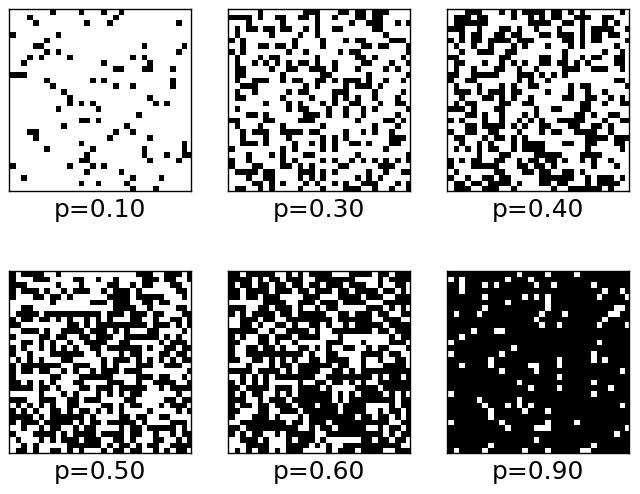
\includegraphics[scale=0.5]{./figures/percolation}
	\caption{Une démonstration de percolation sur une grille à deux dimensions pour différentes valeurs de $p$. Sous le seuil de percolation le système est composé de petites grappes, après un certain point critique $p_c$ une grappe étendue et occupe la grille.}
	\label{percolation}
\end{figure}
\section{Percolation explosive}
En percolation de liaison, on commence de $n$ nœuds non connectés. A chaque pas de temps, un lien est ajouté entre deux nœuds sélectionnés selon une règle donnée. Le nombre des liens ($E$) ajoutés au système à un certain pas de temps divisé par la taille du système est le paramètre de contrôle ($\km=\frac{2E}{n}$) qui décrit la transition de phase. En ce qui concerne le paramètre d'ordre, on peut prendre la fraction des nœuds appartenant à la composante géante du réseau (généralement noté $S(t)$). Au fur et à mesure que le temps augmente, le nombre des liens ajoutés dans le réseau augmente, dans la limite thermodynamique ($N\longrightarrow \infty$), $S(t)$ présente une transition de phase de zéro à $O(1)$ au voisinage d'un point critique ($\km_c$). La percolation classique est une transition de phase géométrique typique, qui a été largement étudiée depuis $1940$ aux nombreux domaines, y compris la mathématique, la physique statistique et l'ingénierie. De nombreux modèles de percolation, tels que la percolation d'invasion, de premier passage,  bootstrap et k-core. 
Tous ces modèles et beaucoup d'autres ont démontré que la transition de phases est étroitement liée à diverses applications, la turbulence, les modèles magnétiques, les colloïdes, la transition de Hall quantique spin, etc. Le lecteur est adressé aux revues récentes dans \cite{Boccaletti-al2016,Souza-Nagler2015,Araujo-al2014}, ses références contiennent un ensemble des principaux résultats et concepts de la percolation classique.\\

Pendant des décennies, la plupart des transitions de la percolation classique (ordinaire) semblent être de type de second ordre (continue) comme la percolation de liaison dans les réseaux ER, pour laquelle la taille de la composante géante augmente progressivement lorsque le paramètre de contrôle, $\km$, dépasse le seuil de percolation. Il convient toutefois de noter qu'il existe également de rares exemples de modèles de percolation présentant une transition de phase de premier ordre (discontinue), tels que la percolation bootstrap \cite{Adler1991}, k-core \cite{Dorogovtsev2-2006} et de brouillage \cite{Echenique-al2005}. Par l'observation que les règles de concurrence non locales ou globales lors des processus de fusion d'amas dans le réseau peuvent conduire à une percolation explosive PE, un certain nombre de ces processus, tels que ceux d'Achlioptas ont été étudiés \cite{Costa-al2010,Costa-al2015,Cho-Kahng2011}.

\subsection{Percolation explosive dans le processus d'Achlioptas}

L'idée principale du processus Achlioptas (PA) \cite{Achlioptas-al2009} est de modifier la règle pour générer des graphes ER. Au lieu d'ajouter des liens aléatoires, dans le processus Achlioptas on choisit deux liens au hasard puis on utilise une règle pour sélectionner l'un ou l'autre. Le lien sélectionnée sera ajouté au graphe alors que l'autre lien sera rejeté. Considérons la Fig.~\ref{achlioptas} (adapté de \cite{Achlioptas-al2009}): (\textbf{A}) l'évolution du réseau  selon le modèle ER, à chaque étape deux nœuds sont choisis au hasard et reliés par un lien (représenté par la ligne pointillée). Dans cet exemple, deux composantes de taille $7$ et $2$ sont fusionnées. (\textbf{B}) Deux liens aléatoires $\{e_1,e_2\}$ sont sélectionnés à chaque étape mais un seul sera ajouté au réseau suivant une règle de sélection, tandis que l'autre sera abandonné.
Soumettant à la règle de produit (RP), le lien sélectionné est celui qui minimise le produit des tailles des composantes qui sont fusionnées. Pour cet exemple, $e_1$ (avec le produit $2\times7=14$) serait choisi et $e_2$ rejeté (parce que $4\times4=16$). En revanche, la règle avec laquelle on sélectionne le lien minimisant la somme des tailles des composantes choisi $e_2$ au lieu de $e_1$. (\textbf{C}) Évolution de fraction de la composante géante  $\frac{C}{n}$ pour: ER, BF (une règle de taille bornée, voir \cite{Bohman-Frieze2001}), et RP. Le réseau étudie est de taille $n=512000$.
\begin{figure}[h!]
	\centering
	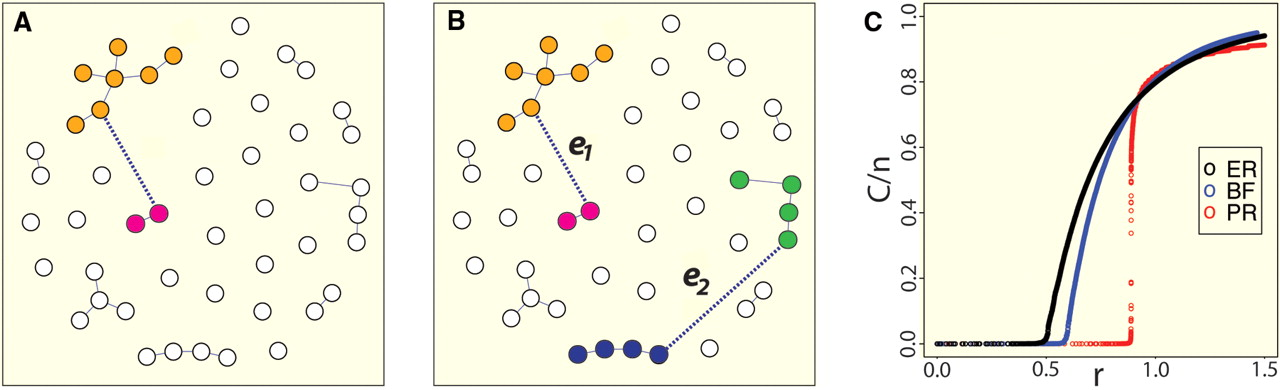
\includegraphics[scale=0.35]{./figures/achlioptas3}
	\caption{Comparaison entre la percolation aléatoire et PA. (\textbf{A}) Percolation ER classique, où les liens sont ajoutés au hasard dans le réseau. (\textbf{B}) Percolation PA, où à chaque étape deux liens sont en compétition pour être établis. (\textbf{C}) Paramètre d'ordre: la taille relative de la composante géante par rapport au nombre des liens ajoutées normalisées par la taille du système.}
	\label{achlioptas}
\end{figure}

Achlioptas s'est demandé s'il est possible de déplacer le point critique de cette transition de phase suivant une règle de sélection appropriée. Une règle qui peut naturellement être imaginée c'est la règle du produit: Parmi les liens donnés, choisir celui qui minimise le produit des tailles des composantes contenant les quatre extrémités de $\{e_1,e_2\}$. Cette règle a été suggérée dans \cite{Bollobas-1984} comme la plus susceptible de retarder le point critique. Une autre règle est la règle de somme, où la taille de la nouvelle composante formée est minimisée. La Fig.~\ref{achlioptas}.(c) est  suffisante pour motiver l'idée pour que la transition de percolation RP soit discontinue. Achlioptas et al. ont utilisé une méthode intéressante pour vérifier que la transition est bien discontinue. Ils mesurent numériquement le pas de temps $t_0$ auquel la taille de la composante géante $(C)$ devient plus grande que $n^{\frac{1}{2}}$ et $t_1$ où $C$ devient plus grand que $\frac{1}{2}\times n$. Un pas de temps correspond à une valeur de $r$ où $r=\frac{E}{n}=\frac{t}{n}$ (puisque le nombre de liens à l'instant $t$ est $E$). Pour le modèle ER et d'autres transitions de percolation continues, on trouve que $\Delta\equiv t_1-t_0$ est extensive, c'est-à-dire il évolue avec $n$. En outre, pour le modèle RP, ils ont trouvé que $\Delta\sim n^{\frac{2}{3}}$. Puisque $\Delta$ est sous-linéaire en $n$, c'est un argument numérique qui montre que dans la limite thermodynamique $n\rightarrow \infty$ la transition de percolation est en effet discontinue.

Cependant, cette conjecture a été rapidement et  rigoureusement désapprouvée par Riordan et Warnke \cite{Riordan-Warnke2011,Riordan-Warnke2012}, en montrant qu'elle ne s'agit pas d'une transition discontinue  mais continue. En effet, leur argument montre des transitions de phase continues pour une classe encore plus grande de processus PA \cite{Riordan-Warnke2012}. Leurs résultats indiquent que la continuité de la transition de phase est une caractéristique si robuste et donc tous les processus Achlioptas ont une transition de phase continue. En revanche, Nagler et ses collègues \cite{Nagler-al2012} ont montré qu'il est également vrai que certains processus de percolation basés sur le choix d'un nombre fixe de sommets aléatoires sont discontinus, et ils ont résolu ce paradoxe apparent. En identifiant et analysant un processus  continu dans le sens défini par Riordan et Warnke \cite{Riordan-Warnke2012} mais qui présente encore un nombre infini de sauts discontinus dans un voisinage arbitraire du point de transition: un escalier du Diable. Il ont démontré analytiquement que la continuité à la première transition de connectivité et la discontinuité du processus de percolation sont compatibles pour certains systèmes de percolations compétitifs.\\

La percolation explosive est un problème scientifique très intéressant dans des champs de recherche plus large que la percolation. Il détient un potentiel considérable pour faire progresser notre connaissance des transitions de phase et des phénomènes critiques. Le fait qu'une légère modification des règles de sélection classiques puisse modifier de manière significative la classe d'universalité de la transition de phase sous-jacente est impressionnant. De plus, il semble que dans des cas extrêmes, l'ordre de transition lui-même puisse également changer.

\subsection{Percolation explosive sous d'autres modèle}
Au-delà de la percolation ordinaire, de nombreux autres modèles ont été développés en basant sur diverses contraintes concernant l'occupation des liens afin de produire PE. Dans ce qui suit, nous examinons brièvement certains de ces modèles suivant de la référence \cite{Boccaletti-al2016}: 
\subsubsection{Les modèles de probabilité}
Ce modèle consiste à donner pour tout amas $i$ un poids $s_i$, pour chaque pas de temps un lien entre une paire des amas $ij$ est occupé par une probabilité proportionnelle à $(s_is_j)^{\alpha}$. La somme  de tous les poids est déterminée comme une constante de normalisation: $w=\sum_i\sum_j(s_is_j)^{\alpha}$, alors la probabilité pour que l'amas $i$ lie avec un autre $j$ est $\frac{(s_is_j)^{\alpha}}{w}$ \cite{Cho-al2010}.\\ Un autre type de ces modèles, c'est le modèle hamiltonien de la référence \cite{Moreira-al2010}, on commence par un réseau de $n$ nœuds sans aucun lien, de sorte que chaque nœud appartient initialement à un amas différent. Tout d'abord, un hamiltonien $H$ simple est défini en fonction des tailles de grappe et du nombre de liens ajoutés à ces grappes. Ensuite, un nouveau lien $e$ entre toute paire de nœuds non encore connectés est ajouté, avec une probabilité proportionnelle à $e^{(-\beta\Delta H_e)}$, où $\Delta H_e$ est le changement d'énergie après l'ajout d'un lien.

\subsubsection{Les modèles Hybrid}
Les modèles hybrides sont ceux pour lesquels la règle d'occupation des arêtes est un mélange de percolation ordinaire et de règles de compétitif: à chaque pas de temps, un lien peut être choisi aléatoirement avec probabilité $p$, alors qu'il peut aussi être choisi suivant une règle de compétitif donnée par la probabilité $1-p$. Par exemple, dans \cite{Bastas-al2014} RP est utilisé, dans la référence \cite{Cao-Schwarz2012} un mélange de $k=2$ et $k=3$-core sur le réseau aléatoire et un mélange de $k=3$-core et des modèles de percolation de brouillage dans le réseau 2D sont étudiés. Les modèles hybrides ont été étudiés dans des réseaux 2D \cite{Cao-Schwarz2012,Bastas-al2014} et des réseaux ER  \cite{Cao-Schwarz2012,Bastas-al2014,Fan-al2012}.
\subsubsection{Les modèles bootstrap}
Dans le cadre du PE, certains modèles bootstrap ont été proposés \cite{Baxter-al2010}. Le processus standard de percolation bootstrap sur un treillis suppose que les sites sont actifs ou inactifs et que l'état d'un site dépend de ses voisins. Initialement, chaque site est activé avec une probabilité $p$, et inactivé avec probabilité $1-p$. Chaque site activé reste dans son état, alors que chaque site inactivé peut devenir actif (et rester actif pour toujours) si ses $k$ voisins les plus proches sont actifs (avec $k=2,3,\ldots$). La procédure est poursuivie jusqu'à ce que le système atteigne la configuration stable qui ne change plus. Dans l'état final du processus, on s'inquiète de savoir s'il existe ou non un groupe géant couvrant de sites actifs. La percolation bootstrap peut montrer des transitions continues ou discontinues, selon le type de réseau et sa dimensionnalité.
\begin{sloppypar}
	
\section{Percolation au voisinage de point critique: approche théorique et simulation}
\end{sloppypar}
\subsection{Introduction}
La détermination de type de transition de phase dans le phénomène de percolation n'est pas encore une science exacte, c'est-à-dire, il n y a pas encore une règle avec laquelle on peut dire que cet ou celle transition est de premier ou de deuxième ordre indépendamment des mécanismes locales d'évolutions de système ou modèle étudié, même que la percolation est l'un des modèles les plus simples et les plus anciens de la physique statistique. Cependant quelque modèles spécifique, par exemple dans \cite{Ziff-al1983}, une approche de l'équation de taux a été utilisée pour déterminer le type de transition de percolation, Par exemple, dans l'évolution des réseaux ER, l'équation de vitesse est écrite dans la limite thermodynamique comme:
\begin{equation}
\frac{\partial n_s(t)}{\partial t}=\sum_{i+j=s}\frac{k_in_i}{c(t)}\frac{k_jn_j}{c(t)}-2\frac{k_sn_s}{c(t)},
\label{ED-5}
\end{equation}
où $c(t)=\sum_{s}k_sn_s$ est la constante de normalisation, $\frac{k_in_i}{c(t)}\frac{k_jn_j}{c(t)}$ est la probabilité qu'une amas de taille $i$ et de poids $k_i$ sera connecte à une amas de taille $j$ et de poids $k_j$ et $2\frac{k_sn_s}{c(t)}$ est la probabilité qu'une amas de taille $s$ et de poids $k_s$ sera connecté à n'import quel amas dans le réseau.\\
Dans \cite{Cho-al2010,Cho2-Kahng2011} les auteures sont généralisé l'Eq.~\ref{ED-5} en prenant $k_i=i^{\omega}$, le cas $\omega=1$ est exactement le cas ER. En utilisant la technique de fonction génératrice, ils ont trouvé l'expression de distribution d'amas au point critique, $n_s(t_c)\sim s^{-\gamma}$, où $\gamma$ est déterminer comme:
\begin{align}
\gamma &=
\begin{cases}
1+2\omega & \text{si}\ 0<\omega<\frac{1}{2} \\
 \frac{1}{2}+\omega& \text{si}\ \frac{1}{2}<\omega<1.
\end{cases}
\label{gama}
\end{align}

En basant sur des simulations numériques, il 'a été trouvé que pour $\frac{1}{2}<\omega<1$ la transition de phase est continue et pour $0<\omega<\frac{1}{2}$ la transition de phase est discontinue. Ainsi, il peut déterminer par simulation le type de transition de percolation dans ce modèle en mesurant l'exposant $\omega$ en termes de processus d'agrégation de cluster. En 1983, un modèle unidimensionnel de percolation a été introduit \cite{Schulman1983} dans laquelle les sites $i$ et $j$ sont reliés par la probabilité $p_{ij}=\frac{p}{\mid i-j\mid^s}$, où $p$ est un paramètre défini dans l'intervalle $0\leq p\leq1$, et $s$ est aussi un paramètre. Dans la référence \cite{Aizenman-Newman1986} les auteurs ont prouvé que la transition est discontinue pour $1<s\leq2$ et ils ont fait d'autres progrès notables associés à la percolation à longue distance, pour plus de détailles voir \cite{Lee-al2016}.\\
Dans ces modèles la caractérisation des transition de phases dépend de certains paramètres intrinsèques  et n'est pas une caractérisation générale qu'on peut appliquer à tous différents modèles de percolation. La question qui se pose, c'est: Est-ce-que possible d'unifier la loi, dont on détermine le type de la transition ? Pour rependre à cette question, il faut d'abord trouver les paramètres ou les grandeurs avec lesquelles on va établir cette unification.\\
Pour cette raison, on propose une méthode qui peut prédire le type de transition de phase au voisinage de point critique. En utilisant la proposition que la distribution d'amas dans le réseau au voisinage de point critique suit toujours une loi de puissance, on définit deux paramètres: le premier est l'exposant $\gamma$ de la distribution d'amas au voisinage de point critique, $P(s)=cs^{-\gamma}$, avec $c$ est la constante de normalisation, et le deuxième paramètre est $\gamma'$ qui dépend de la manière de choisir les amas, plus précisément ce paramètre dépend des corrélations existes dans le réseau, car dans les réseaux corrélés la probabilité de choisir une amas de taille $s$ dans le réseau est différent de sa distribution réel dans le réseau. Par exemple, dans la Fig.~\ref{gama-5} on observe que dans le cas d'un processus Achlioptas, l'exposant de la distribution d'amas avec laquelle les amas se choisissent, $\gamma'$, est différent à la distribution d'amas réel $\gamma=2.5$, par contre dans le cas aléatoire les distributions restent exactement les mêmes, $\gamma'=\gamma=2.5$. Autrement dit, on peut dire que dans les réseaux non-corrélés la probabilité de choisir un amas est exactement lié de sa distribution, qui ce n'est pas le cas dans l'existence des corrélations. D'où on définit la distribution d'amas avec laquelle les amas se choisissent comme $P(s)'=c's^{-\gamma'}$, avec $c'$ est la constante de normalisation.
% En outre, on peut dire que la valeur moyenne des amas choisissent par les liens ajoutés est différents au valeur moyenne des amas dans le réseau, cette  différence de valeur moyenne est similaire au celle dans \cite{Lachgar-Achahbar2016} où les auteurs, en basant sur le degré moyen de nœuds choisi à chaque instant, ont comparé le modèle de BA avec sa complément, le degré moyen utilisé est différent au degré moyen des nœuds usuel. 
 \begin{figure}[h!]
 	\centering
 	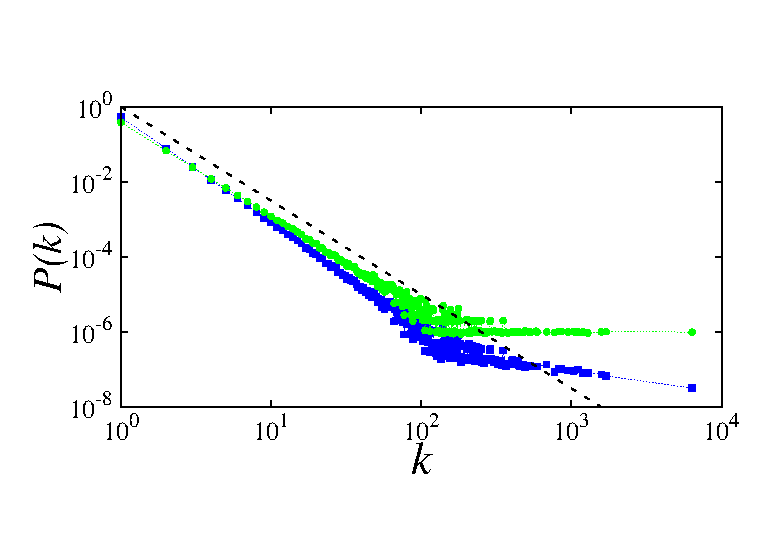
\includegraphics[scale=1.2]{./figures/fig-gama}
 	\caption{La distribution d'amas selon deux méthodes différentes de choisir les liens dans le même réseau, où l'exposant de la distribution d'amas dans le réseau est $\gamma=2.5$, la première méthode est aléatoire comme le processus ER (cercles verts), la deuxièmes est par le processus Achlioptas \cite{Achlioptas-al2009} (carrés bleus). La ligne pointillée a pour but de montrer  l'exposant  $\gamma=2.5$. La taille du réseau est $n=10^6$, chaque simulation est moyennée à $n$ réalisations. }
 	\label{gama-5}
 \end{figure}
 
\subsection{Approche théorique}
\subsubsection{Composante géante:}
Dans cette partie on va élaborer une expression de la composante géante, beaucoup plus générale au celle de ER, au voisinage de point critique en fonction de deux paramètres $\gamma$ et $\gamma'$.
On suppose que le point critique est notre temps initial, puis on ajoute des liens au réseau.
Pour qu'un amas de taille $i$ n'appartient pas à la composante géante, il ne doit pas être connecté à la composante géante via un autre amas de taille $j$. Cela signifie que: (a) l'amas de taille $i$ n'est pas connecté à l'amas de taille $j$ par un lien, ou (b) l'amas  de taille $i$ est connecté à l'amas de taille $j$, mais l'amas de taille $j$ n'est pas lui-même membre de la composante géante.\\
Soit $p=\frac{\km}{n-1}$ la probabilité que deux nœuds se connectent, où
$\km=\frac{2\times\text{(nombre de liens ajoutés)}}{\text{n}}$ est la densité des liens ajoutés par rapport à la taille du réseau.
La probabilité de résultat (a) est $(1-p)^{ij}$, et la probabilité de résultat (b) est $(1-(1-p)^{ij})u$, où $u$ est la probabilité qu'un nœud n'appartient pas à la composante géante. D'où la probabilité qu'une amas de taille $i$ n'appartient pas à la composante géante à travers n'import quelles amas de taille $j$  dans le réseaux est
\begin{eqnarray}
q_{ij}&=&[(1-p)^{ij}+(1-(1-p)^{ij})u]^{n_aP(j)'}\nonumber\\
&\approx&[1-ijp(1-u)]^{n_aP(j)'}\nonumber\\
&\approx&e^{-ijp(1-u)n_aP(j)'},
\end{eqnarray}
 avec $P(j)'=c'j^{-\gamma'}$ est la probabilité de choisir un amas de taille $j$ et $n_a$ est le nombre des amas.
D'où la probabilité qu'un amas de taille $i$ n'appartient pas à la composante géante à travers n'import quels amas est
\begin{eqnarray}
\pi_{i}&=&\prod_{j=1}^{K}q_{ij}\nonumber\\
       &=&e^{-ipn_a(1-u)\sum_{j=1}^{K}jP(j)'},
\end{eqnarray}
où $K=n_a^{\frac{1}{\gamma'-1}}$ est l'amas maximal au voisinage de point critique $(\km_c)$.\\ D'où $\sum_{j=1}^{K}jP(j)'=\kma'$ est le degré moyen avec lequel les amas se choisissent au réseau, ainsi que $\kma$ est la valeur moyen des amas, alors $n=n_a\kma$, et on sait que $p=\frac{\km}{n-1}$, d'où on peut écrire
\begin{eqnarray}
\pi_{i}=e^{\frac{-i(1-u)\km\kma'}{\kma}}.
\label{pi}
\end{eqnarray}
La fraction des amas de taille $i$ qui n'appartient pas à la composante géante par rapport au taille de réseau $n$ est 
\begin{eqnarray}
u_{i}=\frac{n_aiP(i)\pi_i}{n},
\label{ui}
\end{eqnarray}
d'où la fraction des nœuds qui  n'appartient pas  à la composante géante est
\begin{eqnarray}
u=\sum_{i=1}^K u_i.
\end{eqnarray}
Alors la fraction des nœuds qui appartient à la composante géante est 
\begin{eqnarray}
S=1-u=1-\sum_{i=1}^K u_i.
\end{eqnarray}
De Eq.~\ref{pi}, Eq.~\ref{ui} et sachant que $n=n_a\kma$ et $S=1-u$ on obtient
\begin{eqnarray}
S&=&1-\frac{1}{\kma}\sum_{i=1}^KiP(i)e^{\frac{-iS\km\kma'}{\kma}}\nonumber \\
&=& 1-\frac{1}{\kma}\int_{i=1}^KiP(i)e^{\frac{-iS\km\kma'}{\kma}}di.
\label{s}
\end{eqnarray}
 Cette formule au-dessus est une expression beaucoup plus générale à celle de ER \cite{Erdos-Renyi1959}, en effet, dans le cas où on ajoute des liens aléatoirement sans corrélations ,$\gamma=\gamma'$, et lorsque au temps initial tous amas sont de même taille $1$, on va trouver exactement l'expression de ER, $S=1-e^{-S\km}$.
  \begin{figure}[h!]
  	\centering
  	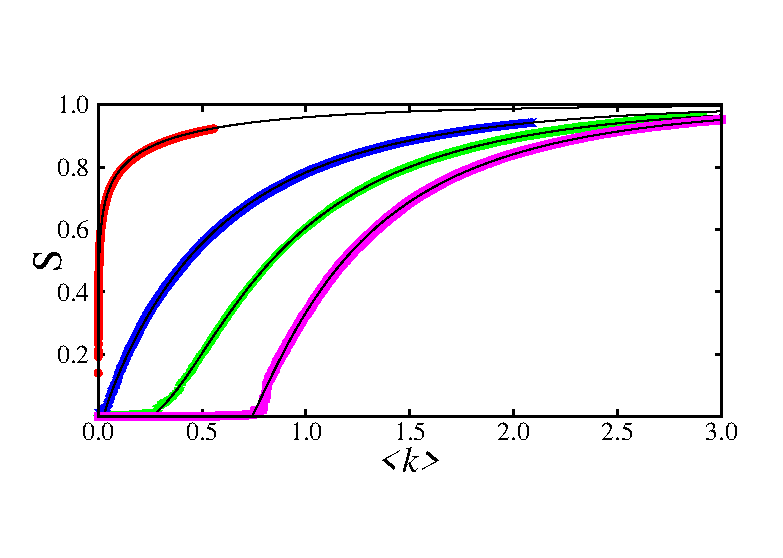
\includegraphics[scale=1.2]{./figures/fig-CG}
  	\caption{Fraction de la composante géante $S$ en fonction de la densité des liens $\km$ pour différents valeurs de $\gamma$, les couleurs de gauche à droite représentent  respectivement les simulations numériques pour $\gamma=2,2.5,3,4$, les lignes noire représentent la solution numérique de l'Eq.~\ref{s}. Le nombre des nœuds est $n=10^5$.}
  	\label{CG}
  \end{figure}
 
 \subsubsection{Détermination de point critique:}
 A partir de Eq.~\ref{s} et en basant sur une solution graphique qui a été utilisé dans \cite{Newman2010-403} on peut obtenir facilement le point critique $\km_c$ où la composante géante  est apparaît, cette méthode s'appuie sur que le point critique $\km$ justifie la condition 
 \begin{equation}
 \frac{\partial (1-\frac{1}{\kma}\sum_{i=1}^KiP(i)e^{\frac{-iS\km\kma'}{\kma}})}{\partial S}\Big)_{S=0}=1,
 \end{equation}
 la solution de cette équation au-dessus nous donne l'expression de point critique suivant
 \begin{equation}
\km_c=\frac{\kma^2}{\kmaa\kma'},
 \end{equation}
 dans le cas où il n'y a pas des corrélations $\gamma=\gamma'$, c'est-à-dire $\kma=\kma'$, on obtient que
  \begin{equation}
  \km_c=\frac{\kma}{\kmaa}=\frac{1}{\kappa_a},
  \label{kc}
  \end{equation}
   cette expression est beaucoup plus exacte de celle donné par \cite{Cho-al2010}, où les auteurs ont trouvé que $\km_c=\frac{1}{\kmaa}$, mais en basant sur les simulations numérique (voir Fig.~\ref{PC} ) il est claire que notre formule est plus exacte.\\
\begin{figure}[h!]
	\centering
	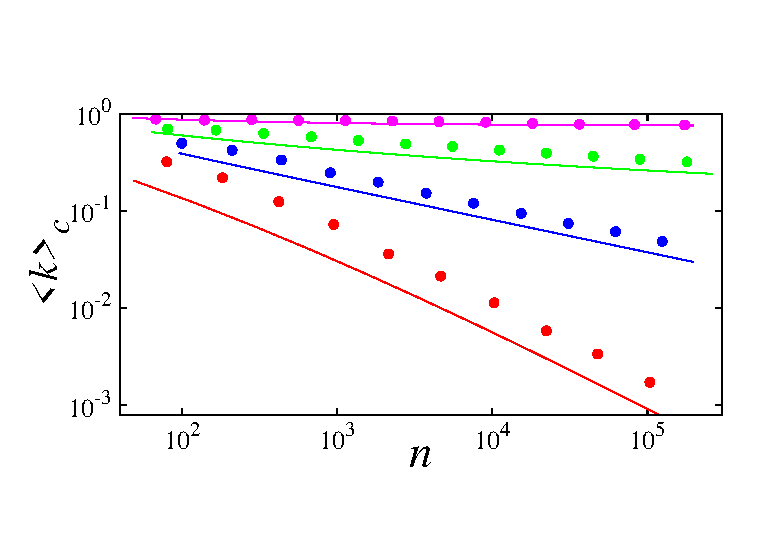
\includegraphics[scale=1.2]{./figures/fig-PC}
	\caption{Estimation de point critique par les simulations numériques (cercles) et par Eq.~\ref{kc} (ligne). Les valeurs de $\gamma$ de haut en bas sont respectivement $4,3,2.5,2$. Chaque simulation est moyennée à $500$ réalisations. }
	\label{PC}
\end{figure}

Il convient de signaler que la détermination de point critique par les simulations n'est pas une opération assez facile, il est un peut compliqué et délicat de le trouvé par une grande précision. Dans nos simulations représentent dans la Fig.~\ref{PC}, nous avons estimé le point critique par la détermination de point où la valeur moyenne des petites amas dans le réseau est maximale,  cependant cette estimation est devient plus pertinent avec l'augmentation de nombre des nœuds du réseau, car les effets d'échelle se diminue avec la taille. Alors on a l'intuition que notre expression théorique est exacte mais le problème est dans la détermination de point critique par les simulations numériques. 
 
 
  \subsubsection{Détermination du type de transition de phase:}
 Pour déterminer le type de transition de phase on va essayer de calculer la valeur de $\km$ pour que $S$ atteindre une valeur à l'échelle macroscopique, $O(1)$, (par exemple $S=\frac{1}{4}$), si $\km$ tend vers zéro on dit alors que la transition est de première ordre sinon on dit qu'elle est au deuxième ordre.\\
 A partir de Eq.~\ref{s} et sachant que $P(i)=ci^{\gamma}$, on obtient
 \begin{equation}
 S=1-\frac{c}{\kma}\int_{i=1}^Ki^{1-\gamma}e^{\frac{-iS\km\kma'}{\kma}}di
 \label{s2},
 \end{equation}
 l'intégrale dans cet expression n'a pas une solution explicite connu, alors il 'est impossible d'extraire la valeur de $\km$ en fonction de $S$,  pour cette raison on propose une autre approche, on va construire la composante géante par la plus vite manière possible, puis on déduit le type de transition de phase selon $\gamma$ et $\gamma'$.\\
 Pour chaque nouveau lien, on lie les deux amas les plus grand dans le réseau\footnote{Cette approche est valable sauf au voisinage de point critique lorsque la distribution d'amas est suit une loi de puissance, car lorsque on commence d'ajouter les liens par cette méthode au loin de point critique, cela peut ralentir  la transition au point critique au lieu de l'accélérer.}, mathématiquement on récrire cela par cette expression 
  \begin{equation}
  S=\sum_{i=1}^tk(t)=\int_{1}^{t}k(i)di,
  \label{s3}
  \end{equation}
  où $t$ représente le temps et également le nombre des liens ajoutés, et $k(t)$ est $t^{\text{ème}}$ degré maximal, avec $k(1)=K$.\\
  $k(t)$ peut être calculer par l'expression suivante
  \begin{equation}
  \sum_{i=k(t)}^Kn_aP(i)=\int_{i=k(t)}^Kn_aP(i)di=t,
  \end{equation}
 d'où on obtient que
   \begin{eqnarray}
   k(t)&=&\Big(K^{1-\gamma}+\frac{(\gamma-1)t}{cn_a}\Big)^{\frac{1}{1-\gamma}}\nonumber\\
     &=& \Big(\frac{t+1}{n_a}\Big)^{\frac{1}{1-\gamma}} \quad \quad  \text{car:} \quad c=\gamma-1 \quad \text{et} \quad K=n_a^{\frac{1}{\gamma-1}} \nonumber\\
     &=& \Big(\frac{t}{n_a}\Big)^{\frac{1}{1-\gamma}}
     \quad \quad  \text{car:} \quad t+1\approx t,
     \label{kt}
   \end{eqnarray}
 de Eq.~\ref{s3} et Eq.~\ref{kt} on trouve que
 \begin{equation}
 S=\frac{\gamma-1}{(\gamma-2)\kma}\Big(\big(\frac{t}{n_a}\big)^{\frac{2-\gamma}{1-\gamma}}-\big(\frac{1}{n_a}\big)^{\frac{2-\gamma}{1-\gamma}}\Big),
 \label{s4}
 \end{equation}
 
 sachant que $\kma=\frac{\gamma-1}{\gamma-2}$ et $t=\frac{n\km}{2}$, on obtient que Eq.~\ref{s4} devient
  \begin{equation}
  S=\Big(\frac{\km (\gamma-1)}{2(\gamma-2)}\Big)^{\frac{2-\gamma}{1-\gamma}}-\Big(\frac{1}{n_a}\Big)^{\frac{2-\gamma}{1-\gamma}},
  \label{s5}
  \end{equation}
  d'où on obtient 
    \begin{equation}
    \km=\frac{2(\gamma-2)}{\gamma-1}\Big(S+\big(\frac{1}{n_a}\big)^{\frac{2-\gamma}{1-\gamma}}\Big)^{\frac{1-\gamma}{2-\gamma}}.
    \end{equation}
  Pour $\gamma>2$ et pour une valeur $S$ donné qui différent au $0$, on peut écrire dans la limite thermodynamique que $ \km=\frac{2(\gamma-2)}{\gamma-1}\Big(S\Big)^{\frac{1-\gamma}{2-\gamma}}$, sous les conditions précédents 
  cette dernière expression ne peut jamais tend vers zéro, ce que signifie absolument que la transition de phase ne peut pas être discontinue pour $\gamma>2$, certes elle est au deuxième ordre, ou plutôt elle est continue.\\
  On a démontré ici qu'il est impossible de trouvé une transition de phase de première ordre, lorsque l'exposant $\gamma>2$ au voisinage de point critique indépendamment de l'autre exposant $\gamma'$, c'est-à-dire indépendamment de corrélations collectives dans le réseau.\\
  Maintenant on va étudier le cas $\gamma=2$ pour déterminer quelle type de transition de phase apparaît ici.\\
   Dans ce cas, l'intervalle de Eq.~\ref{s2} se calcule en s'appuyant sur l'approximation suivante  $e^{\frac{-iS\km\kma'}{\kma}}\approx \frac{1}{1+\frac{iS\km\kma'}{\kma}}$, d'où
  \begin{eqnarray}
  \int_{i=1}^K\frac{i^{-1}}{1+\frac{iS\km\kma'}{\kma}}di&=&\big[ln(i)-ln(i\kmaa\km S+\kma)\big]_{i=1}^{i=K}\nonumber\\
  &=&ln(K)-ln(K\kmaa\km S+\kma)  \quad \quad  \text{car:} \quad K\gg 1,
  \label{appr}
  \end{eqnarray}
  si on remplace Eq.~\ref{appr} dans Eq.~\ref{s2} on obtient 
  \begin{equation}
  S=1-\frac{c}{\kma}\big(ln(K)-ln(K\kmaa\km S+\kma)\big),
  \end{equation}
  d'où l'expression de $\km$ s'écrire
  \begin{equation}
 \km=\frac{e^{\frac{c\ln(K)+\kma(S-1)}{c}}-\kma}{K\kma' S},
  \end{equation}
 sachant que pour $\gamma=2$ on a $K=n_a$ et $\kma=c\ln(n_a)$, on obtient
 \begin{equation}
 \km=\frac{n_a^S-c\ln(n_a)}{n_a\kma' S},
 \end{equation}
  pour $n_a\gg1$ on a $n_a\gg c\ln(n_a)$ et lorsque $S>0$ on peut écrire
  \begin{equation}
  \km=\frac{n_a^{S-1}}{\kma' S},
  \end{equation}
  il est claire que cette expression au-dessus tend toujours vers $0$ pour tous valeurs de $S<1$ et pour n'import quelles valeur de $\gamma'$. Le fait que $\km$ tends vers $0$ cela signifie que la transition est discontinue dans la limite thermodynamique, c'est-à-dire, pour $\gamma=2$ on a une transition de phase de première ordre.\\
  Alors nous avons montrer comment le type de la transition de phase dépend seulement au distribution d'amas au voisinage de point critique (l'exposant $\gamma$), et ne dépend pas des corrélations collectives entre les amas (l'exposant $\gamma'$). \\ 
  En outre, on peut déduire que les corrélations n'ont aucune importance au voisinage de point critique dans la détermination du type de transition de phase, plutôt leur rôle est seulement de mener le réseau à atteindre une certaine distribution d'amas, la transition sera de première ordre si les corrélations réussissent à mener le réseau à atteindre un exposant inférieur ou égale $2$, sinon la transition sera de deuxième ordre. 
\section{Conclusion}
Dans ce chapitre nous avons introduit une méthode pour anticiper  le type de transition de phase dans le phénomène de percolation au voisinage de point critique. Cette méthode basé sur deux paramètres, le premier est l'exposant de la distribution d'amas au voisinage de point critique, $\gamma$, et le deuxième est l'exposant de la distribution d'amas avec lesquels les amas se choisissent, $\gamma'$, ce dernier reflet les corrélations dans le réseau. Nous avons trouvé qu'une transition de phase est de première ordre si $\gamma\leq2$, sinon la transition est de deuxième ordre, indépendamment de la valeur de $\gamma'$.  En outre, on en déduit que les corrélations collectives entre les amas au voisinage de point critique n'ont aucuns influence sur le type de transition de phase, mais elles jouent le rôle pour que le réseau acquérir un certain exposant de distribution d'amas.   

